\begin{figure}[t]
\centering
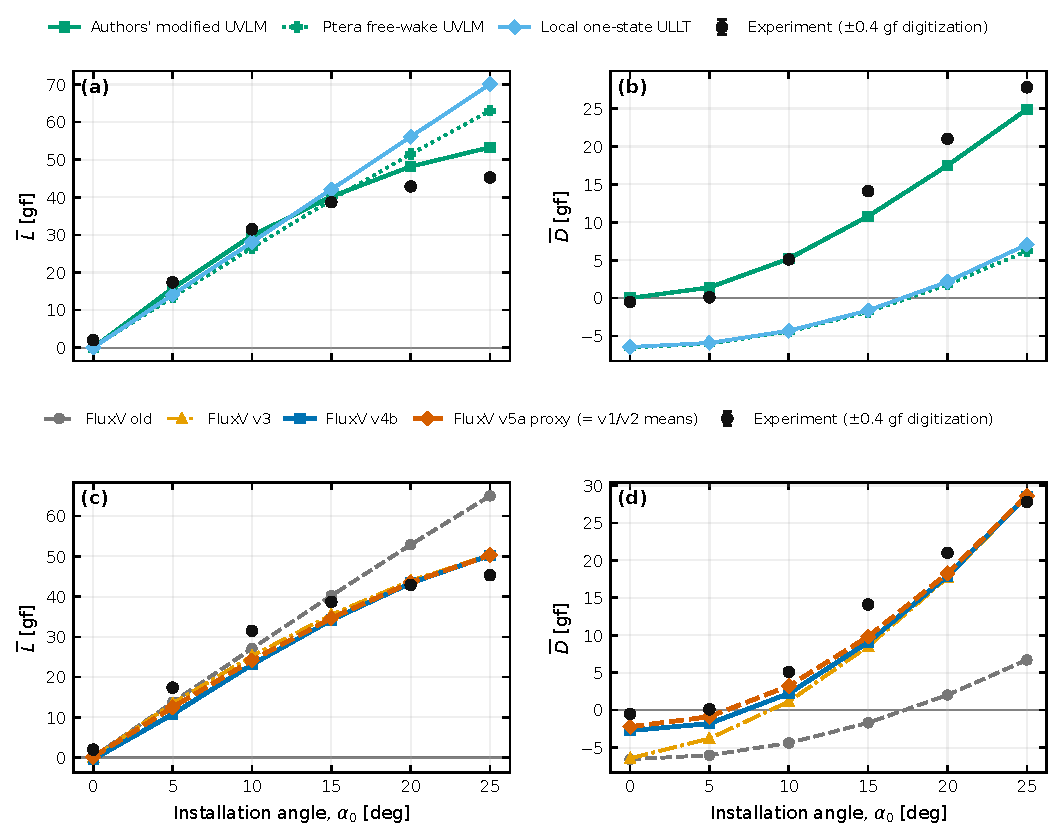
\includegraphics[width=\linewidth]{figures/fig01_yang_all_conditions.pdf}
\caption{Yang et al.全部六个安装角的周期平均升力与有符号阻力。实验误差棒仅表示PDF数字化不确定度（±0.4 gf），不是实验置信区间。论文没有公开相位载荷，故本图不作相位精度声明。v5a是被否决的development proxy，其六点均值与v1/v2重合；v5b未进入跨论文评分。}
\label{fig:fig01_yang_all_conditions}
\end{figure}

\begin{figure}[t]
\centering
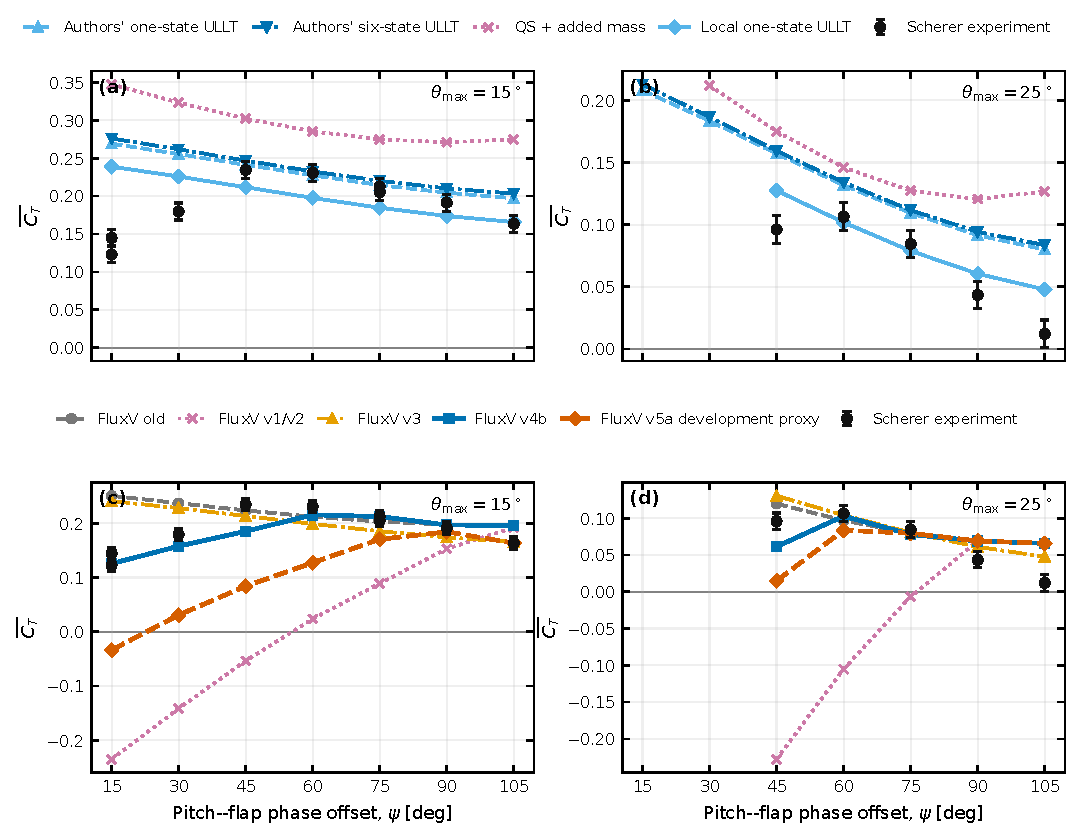
\includegraphics[width=\linewidth]{figures/fig02_izraelevitz_fig14_all_conditions.pdf}
\caption{Izraelevitz/Scherer Figure 14全部公开工况。黑点保留14个原始实验观测，包括两个重复测量；FluxV指标另同时报告12个唯一工况口径。作者在theta=25 deg、psi=15/30 deg的参考点没有实验支持，不参与评分。误差棒为数字化的原图报告条，其统计含义未公开。}
\label{fig:fig02_izraelevitz_fig14_all_conditions}
\end{figure}

\begin{figure}[t]
\centering
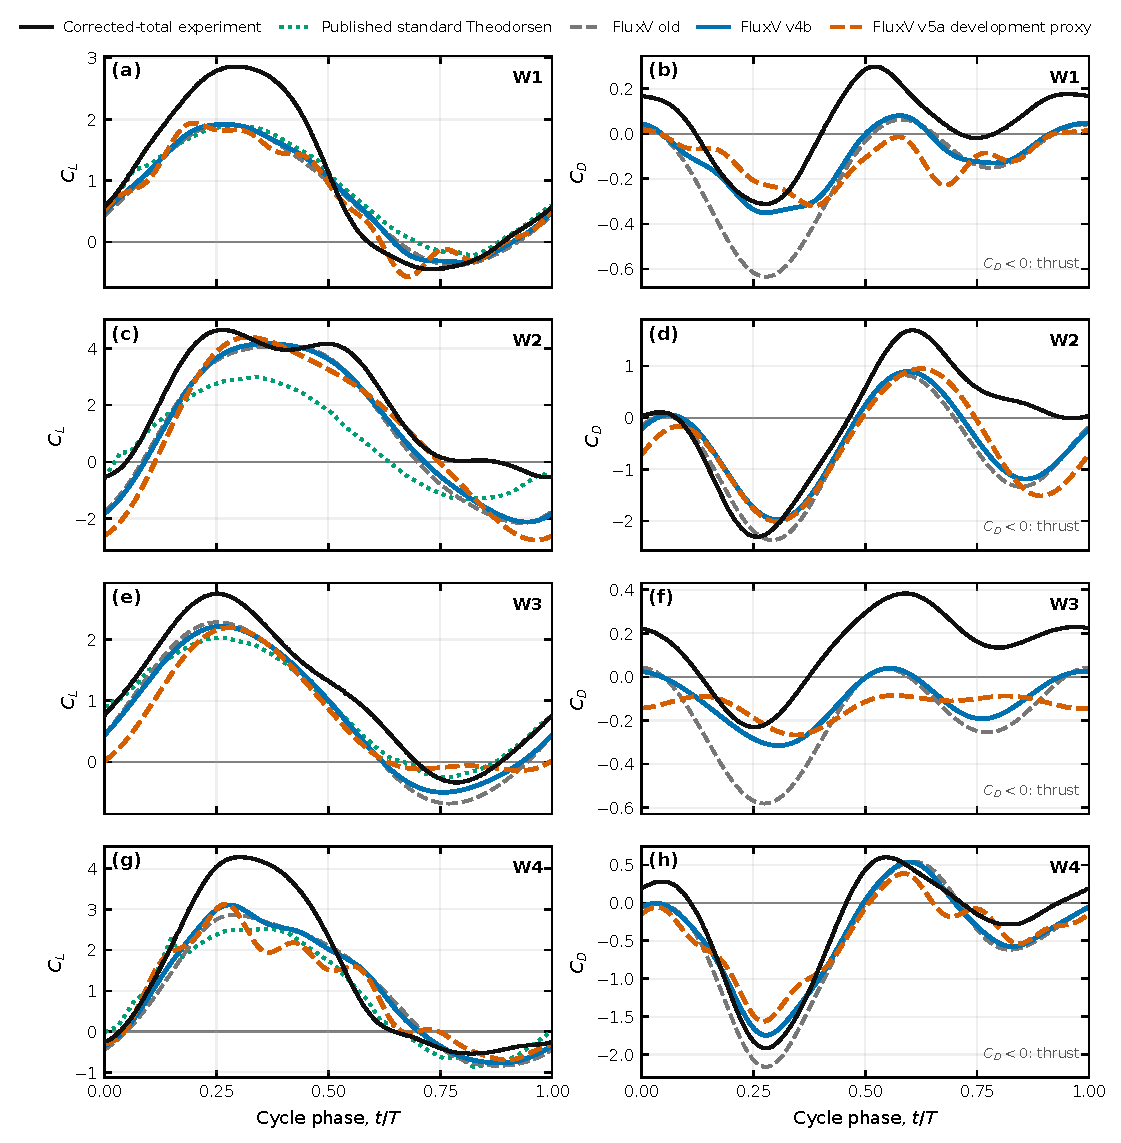
\includegraphics[width=\linewidth]{figures/fig03_baik_w1_w4_filtered.pdf}
\caption{Baik W1--W4全部相位升阻力，采用与原文1 Hz处理相匹配的模型滤波：W1/W4保留至第7谐波，W2/W3保留至第3谐波；每工况评分400个唯一相位点，不做相位、幅值、均值或偏置拟合。负CD表示推力。Theodorsen仅有升力参考。}
\label{fig:fig03_baik_w1_w4_filtered}
\end{figure}

\begin{figure}[t]
\centering
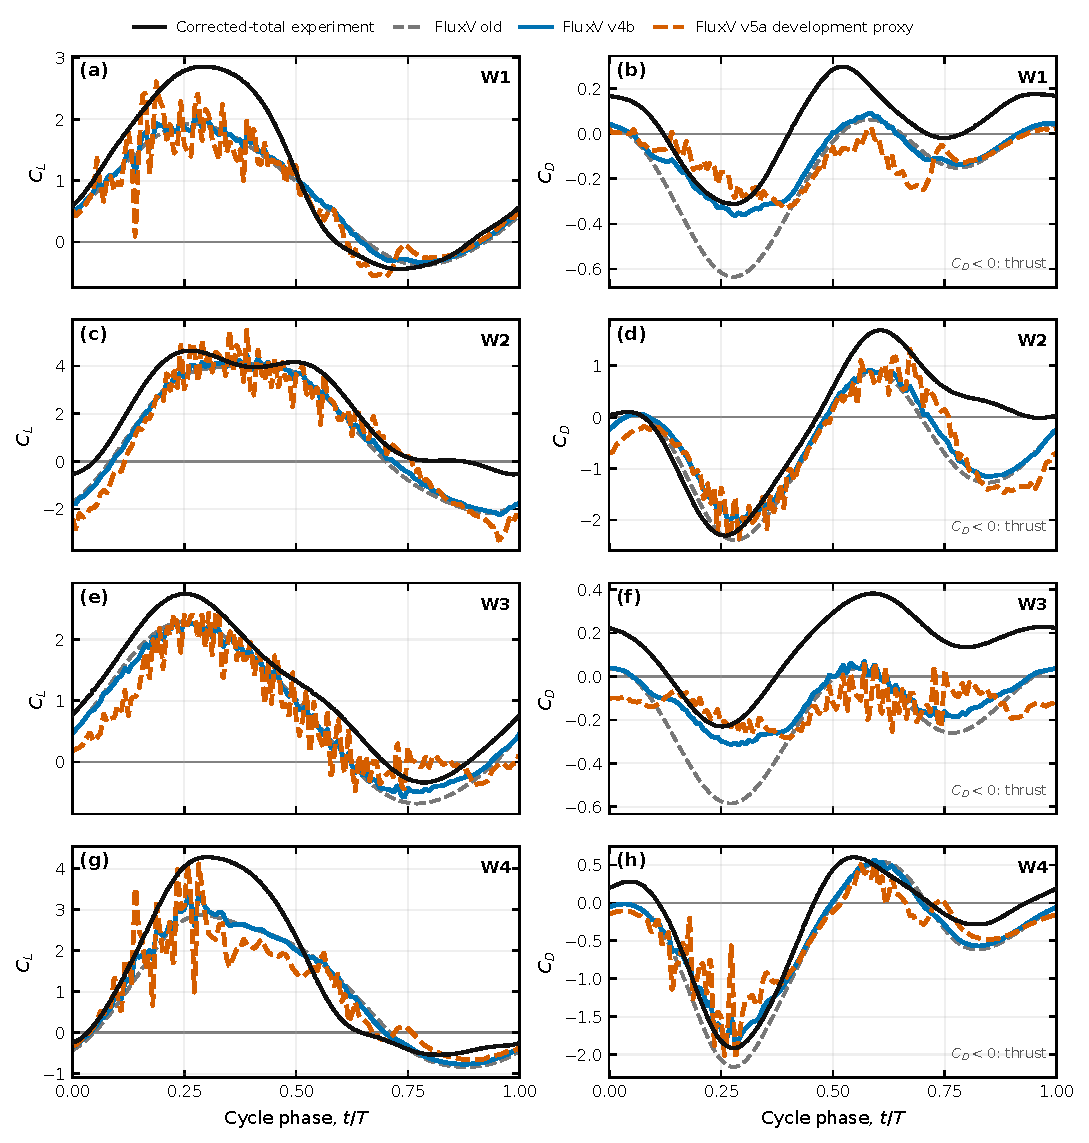
\includegraphics[width=\linewidth]{figures/figS01_baik_w1_w4_raw_numeric.pdf}
\caption{Baik未滤波数值预测的补充诊断。公开实验曲线本身已经过1 Hz处理，因此该图只用于暴露数值模型的高频内容，不是raw-experiment验证，也不作为主精度排序口径。}
\label{fig:figS01_baik_w1_w4_raw_numeric}
\end{figure}

\begin{figure}[t]
\centering
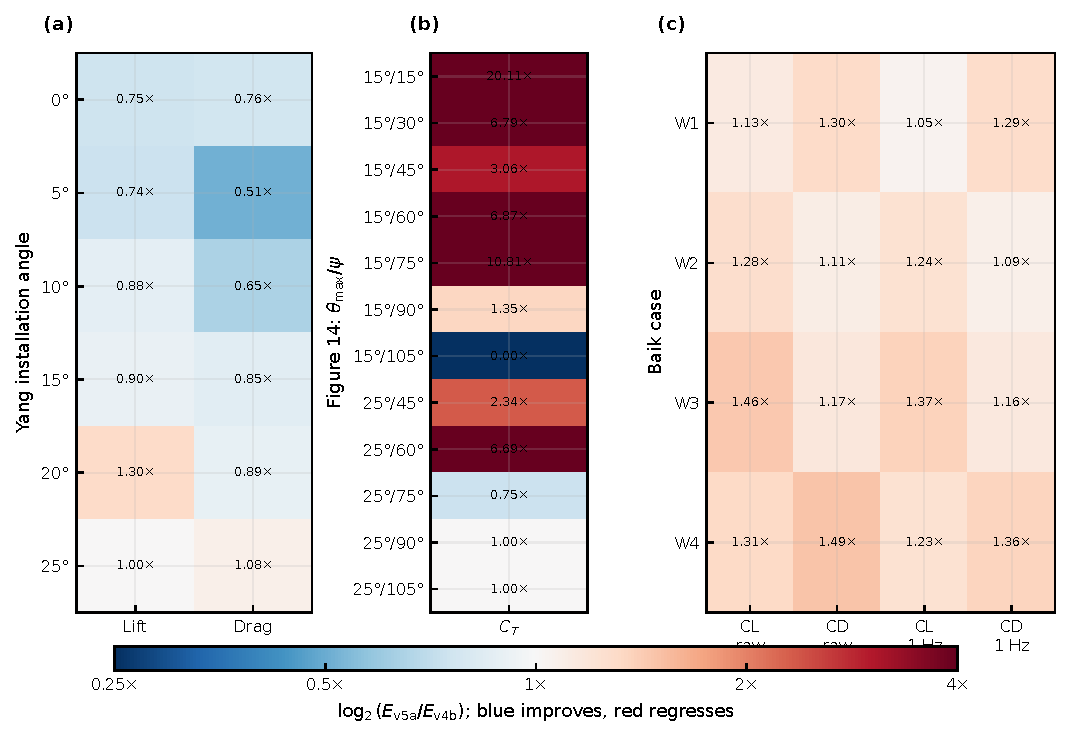
\includegraphics[width=\linewidth]{figures/fig04_all_condition_error_ratio.pdf}
\caption{全部工况逐项v5a/v4b误差比。Yang与Figure 14采用逐工况绝对误差，Baik采用每个W工况的相位RMSE；颜色是log2比值，格内标实际比值。蓝色小于1为改善，红色大于1为退化，不跨物理单位汇总。}
\label{fig:fig04_all_condition_error_ratio}
\end{figure}

\begin{figure}[t]
\centering
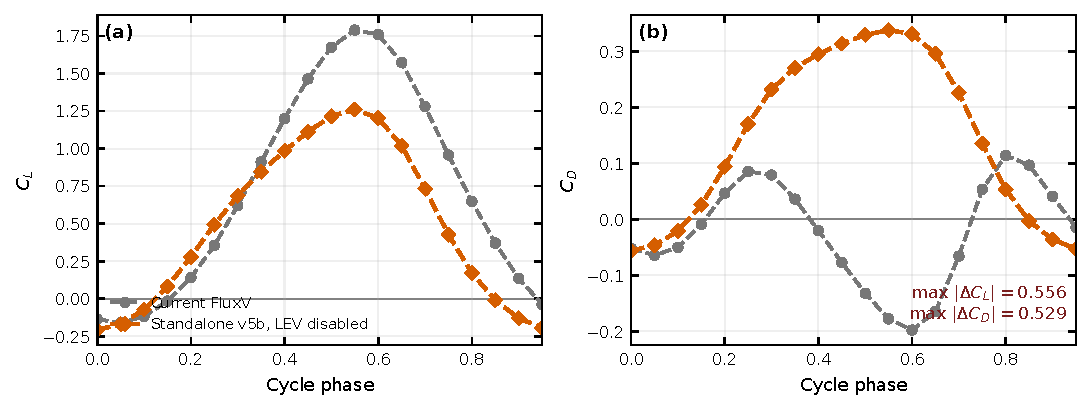
\includegraphics[width=\linewidth]{figures/fig05_v5b_no_lev_gate.pdf}
\caption{v5b进入三论文评分前的no-LEV精确退化门。共同Yang 15 deg运动下，全周期没有活跃LEV，但standalone v5b仍与current FluxV相差max abs dCL=0.556、dCD=0.529；因此v5b被阻断且没有三论文全工况曲线。本图是实现门控诊断，不是实验验证。}
\label{fig:fig05_v5b_no_lev_gate}
\end{figure}
